%%%%%%%%%%%%%%%%%%%%%%%%%%%%%%%%%%%%%%%%%%%%%%%%%%%
%
%  New template code for TAMU Theses and Dissertations starting Fall 2012.  
%  For more info about this template or the 
%  TAMU LaTeX User's Group, see http://www.howdy.me/.
%
%  Author: Wendy Lynn Turner 
%	 Version 1.0 
%  Last updated 8/5/2012
%
%%%%%%%%%%%%%%%%%%%%%%%%%%%%%%%%%%%%%%%%%%%%%%%%%%%

%%%%%%%%%%%%%%%%%%%%%%%%%%%%%%%%%%%%%%%%%%%%%%%%%%%%%%%%%%%%%%%%%%%%%%%
%%%                           SECTION II
%%%%%%%%%%%%%%%%%%%%%%%%%%%%%%%%%%%%%%%%%%%%%%%%%%%%%%%%%%%%%%%%%%%%%%

\chapter{\uppercase {Productivity \& Performance Analysis}}
The main goals of SAC are productivity and performance, but how to measure them? Programming productivity \cite{ProgramProductWiki} refers to software development issues and methodologies affecting the quantity and quality of code produced by an individual or team. The principal factors that affect productivity include learning curve (how friendly of user interface and compatibility with existing software), speed of code generation (how many lines of codes need to write) and approach to testing and maintenance (the running time at which user need to wait and debug methods). For performance issue, the executation times and job scheduling policy play key roles. The performance of a system also involves one or more characteristics such as response time, throughput, utilization of computing resources, availability or bandwidth etc. In this thesis, the (Lines of Codes) LOCs to accomplish same task and friendly user interface are discussed for measuring productivity, while executation time (speedup to sequential codes) and throughput are used for measuring performance.  

\section{Productivity Analysis}
The computer had developed from single core to multicores, but most programmers did not catch up with this trends on time. Our thinking is custom to single thread and single process applications, especially for other domain experts who did not major in computer science. For most application developers, the main tasks of programming models are trying to hide the sophisticated details and making them easy to use. To shorten the learning curve, SAC provide friendly web interface in which user only need to select and coding with template, and all other details such as data distributation, task parallization and scheduling are transparent to user. In the view of end user, only code snippet of core algorithm need to compose, so it is even simpler than writing sequential codes. To improve usibility, Breeze also provides similar operators to those in Matlab and Numby as show in Table \ref{tab:BreezeOperators}, and all of those could be used directly in template codes of SAC. In Figure \ref{}, it gives rough comparision of LOCs calculator in sequential codes, parallel codes with MPI and template codes with SAC. Since the outlines of most seismic applications are similiar, we could divide them into serval categories and abstract commonly used templates. With templates, the outline codes could be resused by all programms in same category, thus make them easy to maintain.   


%A table example is going to follow.
\begin{table}[H]
\centering
\caption{Operators in Breeze, MATLAB and Numpy}
\begin{tabular}{||l|l|l|l||}
\hline
Elementwise addition & a + b & a + b & a + b \\
\hline
Elementwise multiplication & a :* b & a .* b & a * b \\
\hline
Elementwise comparison & a :\textless{}  b & a \textless{}  b & a \textless{}  b \\
\hline
Inplace addition & a :+= 1.0 & a += 1 & a += 1 \\
\hline
Inplace elementwise multiplication & a :*= 2.0 & a *= 2 & a *= 2 \\
\hline
Vector dot product & a dot b & dot(a,b)	& dot(a,b) \\
\hline
Elementwise sum	& sum(a) & sum(sum(a)) & a.sum() \\
\hline
Elementwise max & a.max & max(a) & a.max() \\
\hline
Elementwise argmax & argmax(a) & argmax(a) & a.argmax() \\
\hline
Ceiling	& ceil(a) & ceil(a) & ceil(a) \\
\hline
Floor	& floor(a) & floor(a) & floor(a) \\
\hline
\end{tabular}
\label{tab:BreezeOperators}
\end{table}
%%%%%%%%%%%%%%%%%%%%%%%%%%%%%%%%%%%%%%%%%%%%%%%%%%%%%%


\section{Performance Analysis}
There are a lot of tools used for measuring performane of application. To get the executation time, wall clock is the simplest way. But if we want to make some deep analysis to find the bottleneck, more information such as CPU usage, memory usage, disk I/O and network communication metrics need to be collected. The situation becomes more complex if application run in multithread or run on multinodes with synchronization. Spark itself provide web UI for monitoring of resource usage of whole cluster, task running status and detail of each stage in task. Nigel's performance Monitor (nmon) could collect miscellaneous metrics information on each node, and Nmon Analyzer could visualize such information for deep analysis. So we use wall clock to get total running time and executation of each stage for sequential codes, and use Spark web monitor UI to get executation time of parallel codes running on Spark. Each node will launch nmon to collect runtime information at the same time of application starts, and then all of these data are merged together, feed to Nmon Analyzer for deep study. 

%%%%%%%%%%%%%%%%%%%%%%%%%%%%%%%%%%%%%%%%%%%%%%%%%%%%%%%
\begin{figure}[H]
%\centering
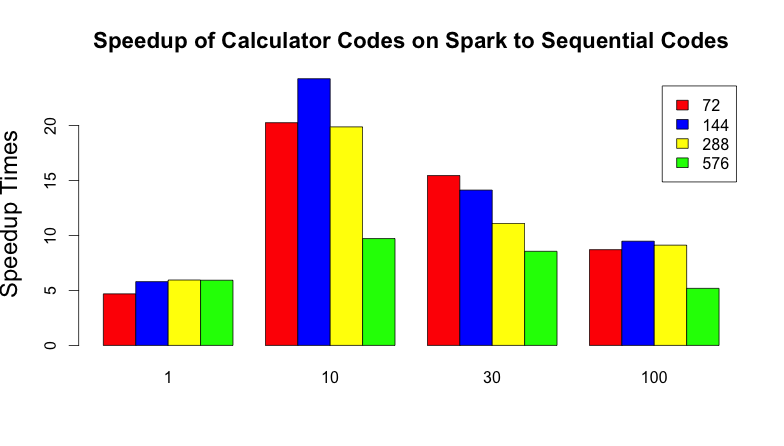
\includegraphics[scale=.60]{figures/CalcSpeedup.png}
\caption{Speedup of Calculator Codes}
\label{CalcSpeedup}
\end{figure}
%%%%%%%%%%%%%%%%%%%%%%%%%%%%%%%%%%%%%%%%%%%%%%%%%%%%%%%
 

%%%%%%%%%%%%%%%%%%%%%%%%%%%%%%%%%%%%%%%%%%%%%%%%%%%%%%%
\begin{figure}[H]
%\centering
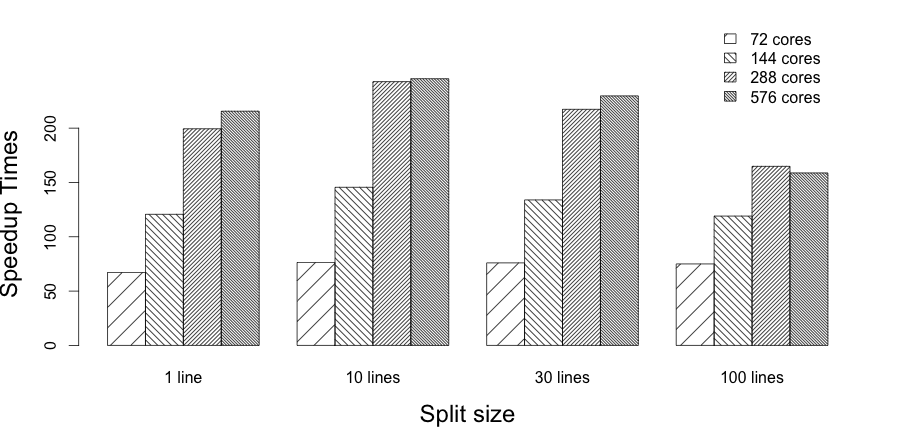
\includegraphics[scale=.60]{figures/HtfSpeedup.png}
\caption{Speedup of Hilbert Transform Filter Codes}
\label{HtfSpeedup}
\end{figure}
%%%%%%%%%%%%%%%%%%%%%%%%%%%%%%%%%%%%%%%%%%%%%%%%%%%%%%%


%%%%%%%%%%%%%%%%%%%%%%%%%%%%%%%%%%%%%%%%%%%%%%%%%%%%%%%
\begin{figure}[H]
%\centering
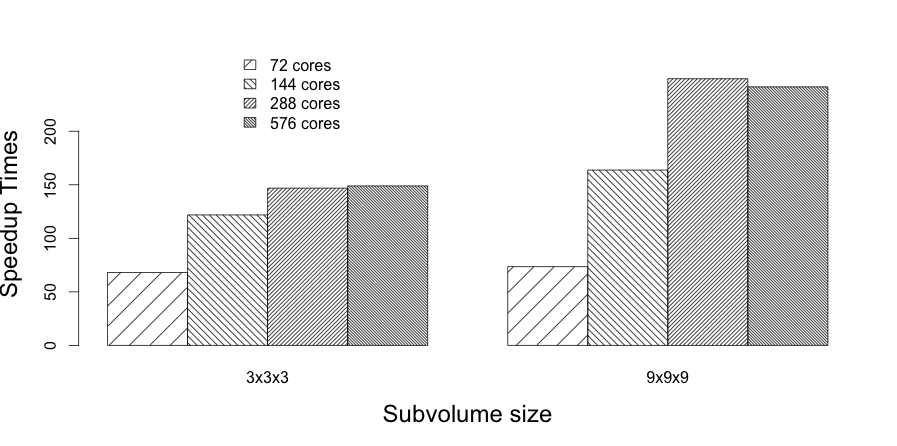
\includegraphics[scale=.60]{figures/FFTSpeedup.png}
\caption{Speedup of FFT Codes}
\label{FFTSpeedup}
\end{figure}
%%%%%%%%%%%%%%%%%%%%%%%%%%%%%%%%%%%%%%%%%%%%%%%%%%%%%%%

%%%%%%%%%%%%%%%%%%%%%%%%%%%%%%%%%%%%%%%%%%%%%%%%%%%%%%%
\begin{figure}[H]
%\centering
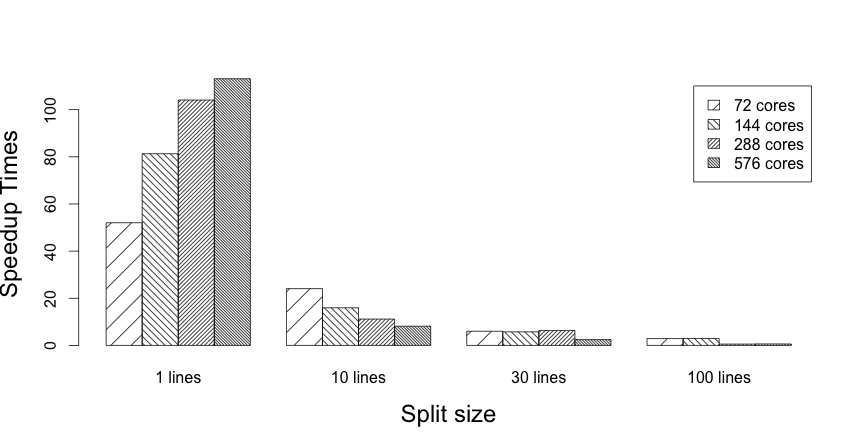
\includegraphics[scale=.60]{figures/HistSpeedup.png}
\caption{Speedup of Histogram Computation Codes}
\label{HistSpeedup}
\end{figure}
%%%%%%%%%%%%%%%%%%%%%%%%%%%%%%%%%%%%%%%%%%%%%%%%%%%%%%%


%%%%%%%%%%%%%%%%%%%%%%%%%%%%%%%%%%%%%%%%%%%%%%%%%%%%%%%
\begin{figure}[H]
%\centering
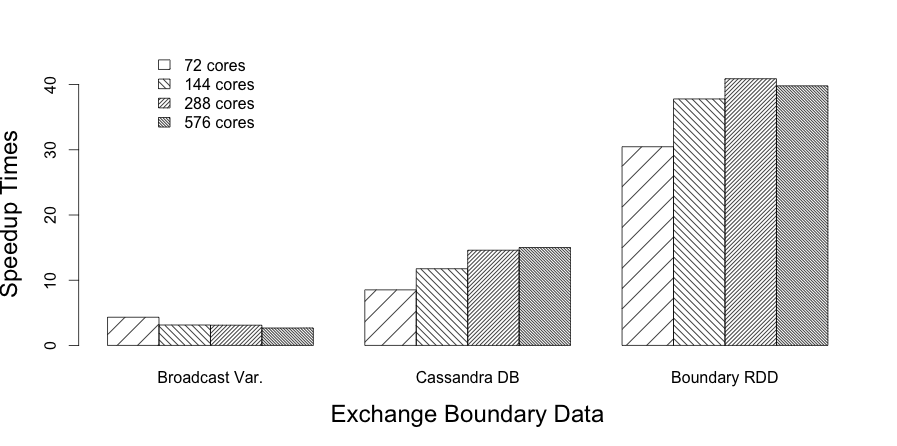
\includegraphics[scale=.60]{figures/JacobiSpeedup.png}
\caption{Speedup of Jacobi Stencil Codes}
\label{JacobiSpeedup}
\end{figure}
%%%%%%%%%%%%%%%%%%%%%%%%%%%%%%%%%%%%%%%%%%%%%%%%%%%%%%%

Due to space limitations, we only select two typical application for analysis: one is Hilbert tranformation on trace template, the other is Jacobi stencil codes on subvolume case.

\subsection{Performance Analysis of Hilbert tranformation}
 

\subsection{Performance Analysis of Jacobi iteration}




